\documentclass[a4paper,man,natbib,floatsintext]{apa6}

\usepackage[english]{babel}
\usepackage[utf8x]{inputenc}
\usepackage{amsmath}
\usepackage{graphicx}
\usepackage[colorinlistoftodos]{todonotes}
\usepackage[font=small,labelfont=bf]{caption}
\newcommand{\rpm}{\raisebox{.2ex}{$\scriptstyle\pm$}}
\usepackage{amsmath}
\DeclareMathOperator*{\argmax}{arg\,max}

\title{Sherlock topic model paper}
% A common space for dynamic experiences and memories
% Geometric principles of episodic recall for naturalistic experiences
% The geometry of episodic recall for naturalistic experiences
% Recasting episodic memory as a weighted blend of prior experiences
% Capturing the moment-by-moment flow of information in naturalistic stimuli
% A continuous, content-general approach to characterizing memory for naturalistic events
% A common model for naturalistic stimuli, memories, and brains
% \title{A dynamic, content-general encoding signal to characterize memory for naturalistic stimuli}
% Topic models as a bridge between naturalistic stimuli, memories, and brains
% Automated analysis of memory for naturalistic stimuli using topic modeling
% Topic modeling as a link between videos and memories
% Topic models as a bridge between dynamic experiences and memories

\shorttitle{Your APA6-Style Manuscript}
\author{Andrew C. Heusser \& Jeremy R. Manning}
\affiliation{Dartmouth College}

\abstract{
}

\begin{document}
\maketitle

\section{Introduction}

- using list-learning / trial based experiments, we've learned a great deal about the human memory system.
- however, its undeniable that many lab-based experiments are severely contrived as compared to real life experiences
- for example, real life experiences are typically highly autocorrelated in space and time, a feature that is not typically present in traditional laboratory studies.
- nonetheless, we want to leverage the tools and knowledge gained over the past few decades
- here, we present a methodological and theoretical advance in our understanding of memory for naturalistic experiences.
- our approach is model the semantic information contained in a stimulus and project memory responses into this stimulus space, allowing for fine-grained analysis of the mnemonic reprsentations.

\subsection{Results}

\begin{figure}[t!]
\centering
\includegraphics[width=1\textwidth]{figs/0_analysis_schematic.pdf}
\caption{\label{fig:schematic}Schematic of the analysis approach. For each moment of the video, text descriptions were manually generated. Three exemplary time points are displayed here.  Below the video descriptions are text samples from an example participant's verbal recall transcript.  We trained a topic model on the moment-by-moment video description text and transformed participant's recall transcripts using this same model. The bar charts display the resulting topic model weights for the video (in blue) and recall (in orange) for three example topic dimensions.}
\end{figure}

\subsubsection{A model to capture the moment-by-moment flow of information in naturalistic stimuli}
We fit a topic model to overlapping windows of manually annotated text descriptions of scenes from an episode of the BBC series, Sherlock. The text description contained details of the scene such as the characters, location, and a short summary of the scene (see \ref{fig:schematic} for example text, see \ref{sec:methods} for analysis details). We then transformed the text descriptions with the (same) topic model, resulting in a scenes (1000) by topics (100) matrix where each row of the matrix represents a probabalistic mixture of topics discovered in that scene. We expanded this matrix from 1000 to 1976 timepoints by copying the vectors for scenes that spanned multiple TRs. As depicted in \ref{fig:model}a, the topics are sparse and change slowly over time. This gradual change was anticipated, since we used overlapping windows of text (50 sentences) as input to the model. The sparsity was also expected since the topic modeling approach we used (Latent Dirichlet Allocation) assumes a sparse Dirichlet prior. By eye, there are clear transitions from one topic `state' to the next, likely indexing scene transitions in the stimulus.  To get a better handle on this temporal structure, we computed the timepoint-by-timepoint correlation matrix of the video model (\ref{fig:model}b).  This correlation matrix reveals that the model has a strong, blocky structure along the diagonal.  Another interesting feature is that there is very little correlation between events (i.e. the off-diagonal values are small). This is an important feature of the model because the `event' representations are unique and highly discriminable.

\subsubsection{Projecting verbal recall into stimulus space}
After watching the episode, participants verbally recalled (in order) as much of the episode as they could.  We used the same topic model (fit with the text descriptions of the video) to transform participants' verbal recall transcripts (split by sentence in overlapping chunks of 10 sentences). The result was a sentences (range: X to X) by topics (100) matrix for each participant, where each row represented the estimated mixture of topics for a given window of sentences during recall. In order to average the recall models across participants, we resampled each model at the resolution of the video model (1976 timepoints). The individual models can be seen in Supp Fig X and the group average is plotted in \ref{fig:model}c. Note that the topics were derived solely from the text descriptions of the stimulus, and so the topic models estimated for recall are entirely dependent on the topics in the episode. In effect, this approach projects the participants' verbal recall into the video 'stimulus space', allowing us to quantify the dynamics of verbally reported memories as well as relate them to the experiences from which they were born.

Next, we investigated the temporal structure of the recall matrices. For each participant, we computed a timepoint-by-timepoint correlation matrix from recall models. Like the video model, the recall correlation matrices exhibited blocky structure along the diagonal (Supp Fig X). To visualize the group average, we resampled all of the recall models to the duration of the video model (1976 timepoints), computed the timepoint-by-timepoint correlation matrices and then averaged across partcipants.  Like the video correlation matrix, the average recall matrix was blocky along the diagonal, albeit noisier (\ref{fig:model}d).  Presumably this noise stems from the fact that there was variability in the amount of time each participant spent describing each event. We will come back to this point later in the paper.

\subsubsection{Correlating the video and recall models}
The participants in this study were instructed to recall as much of the episode as they could in the order it happened.  Thus, we expected that to the extent that participants followed these instructions and had reasonably good memory accuracy, the recall models should resemble the video model. In our first approach to test this hypothesis, we correlated each moment of the video model with each moment of each participants' resampled recall model. We then averaged these matrices together to get a single group averaged matrix.  The result was a viewing time (1976) by recall time (1976) correlation matrix representing the average relationship between every moment of the movie and recall models (\ref{fig:model}e). Notably, we observe significant correlation values (p<.05, permutation test described in \ref{sec:methods}) primarily along the diagonal, suggesting that our model captures the fact that participants recalled the episode in order. We also visualized this effect by projecting the matrices into a 3D space (reduced using Spectral Embedding [cite]) where the proximity of the trajectories at every timepoint represents how similar the topic vectors were. Visualizing the data in this way makes it clear that the overall shape and correlational structure of the video and average recall matrices is quite similar.

\begin{figure}[t!]
\centering
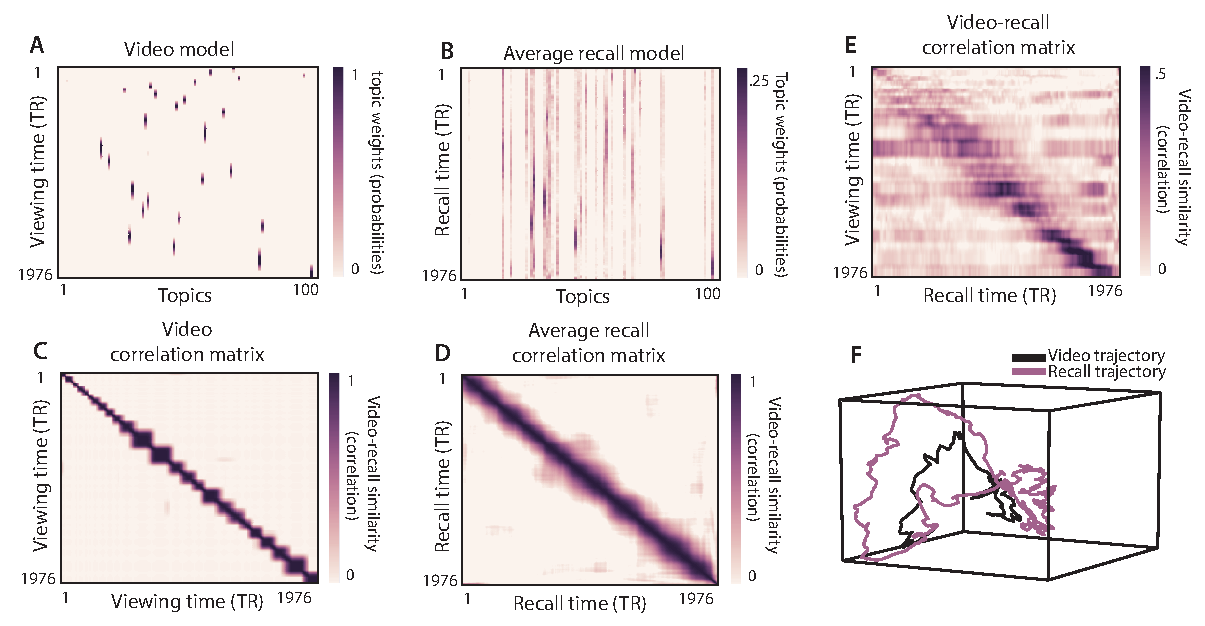
\includegraphics[width=1\textwidth]{figs/1_video_recall_models.pdf}
\caption{\label{fig:model}Topic models for the video and verbal recall. A. A timepoints (1976) by topics (100) matrix was created by fitting a topic model to overlapping segments of the moment-by-moment video text descriptions.  Each row represents the most likely mixture of topics for a given timepoint. Each columns represents a different topic. The darker the color, the higher the probability that the topic is contained in that timepoint. B. A timepoints (1976) by topics (100) matrix representing group average topic model of the recall transcripts.  All participant's recall transcripts were transformed using the topic model fit to the video descriptions and then resampled to the same length (1976). C. A viewing-time (1976) by recall-time (1976) correlation matrix representing the correlation of each moment of the video model with every moment of the average recall model. The darker the color, the higher the correlation between the video and recall models at a given timepoint. D. A 3D embedding of the video and recall topic models reduced using spectral embedding. }
\end{figure}

\subsubsection{Segmenting the video and recall models into events}
One prominent feature of the video and recall correlation matrices (see \ref{fig:model}) is the strong, blocky structure along the diagonal.  We hypothesized that this structure arises from transient stability in the language used to describe each event of the video. If that were true, we reasoned that it would be possible to decode which particular event a participant is describing by comparing the average topic model for a particular recall `event' with the average topic vector for each video event. The video event that is most similar to the given recall event is the event the participant is most likely describing.  To test this idea it is first necessary to systematically parse the matrices into events.  To do this, we leveraged the event segmentation approach developed by Baldassano et al 2017.  Briefly, this algorithm implements a variant of a Hidden Markov Model to estimate k events given a (multivariate) time series and a k value (number of states). We automatically determined a k value for the video model and each participant's recall model using the following equation:

% ADD EQUATION HERE

The algorithm determined 34 events for the movie model and a range of values (range=8-27, mean= 15.41, SD=5.6) for the recall models.  The events discovered for a representative participant can be seen in \ref{fig:eventseg}b. Importantly, the k values were highly correlated to hand annotated accuracy (r(16)=.67, p=.003) across participants. Thus, the blocky temporal structure in the recall matrices computed by our model is strongly related to the variability in memory performance across participants.

Next, we tested the hypothesis that the individual `blocks' along the diagonals of the recall matrices represent the recall of a particular video event. To this end, first we created a video event model, which was done by averaging together neighboring topic vectors that the were classified to be in the same event (\ref{fig:eventseg}c), resulting in an events (34) by topics (100) matrix.  We performed the same procedure for the recall matrices (see \ref{fig:eventseg}d for example). Then, we computed the correlation between these two event models, resulting in a video events (34) by recall events (8-27, depending on the participant) correlation matrix (see \ref{fig:eventseg}e). These matrices represent the extent to which each recall event is similar to each video event (for each participant). To determine which video events the recall events most likely referred to, for each recall event, we found the index of the video event with the highest correlation (i.e. the argmax).  This is depicted in \ref{fig:eventseg}e as the cell highlighted with the black box for each column in the video-recall event correlation matrix. Notably, our algorithm suggests that the example participant recalled the events largely in order, occasionally skipping over an event.

Next, we computed a group average recall event model and video-recall event correlation matrix (\ref{fig:eventseg}f).  To do this, for each participant (and each recall event), we grouped the recall event vectors by the video event that they were most highly correlated to. We then averaged the recall event vectors across subjects. This gave an average recall event vector for all but one (of 34) events since no subjects remembered this events (according to our model). Lastly, we computed an average recall event (34) by video event (34) correlation matrix, and highlighted the highest correlation in the column with a black box (\ref{fig:eventseg}f). Notably, this matrix displayed high correlation values along the diagonal and low correlations in the off-diagonal cells.

To better visualize the relationship between the video and recall models, we embedded the video and average recall model into a 2D space (using the UMAP dimensionality reduction algorithm, for details see \ref{sec:methods}) where the points represent video/recall events and the distance between them represents their similarity in 'topic space' (\ref{fig:eventseg}g). We computed the group average transition probabilites from each event to each other event and plotted the values as lines where the tranparency is proportional to the probability of the transition.  By eye, it is clear that the two models have a very similar geometric structure, and the transition probabilities tend to be strongest between events that occured sequentially (or nearby) in time.

To explore individual variability (and consistency) in the recall event models, we embedded each participant's recall event model in the same 2D 'topics space' described above (\ref{fig:eventseg}h). Despite the variability in the number of events remembered, the overall shape of most of the participants' recall trajectories are similar to the video model (\ref{fig:eventseg}h), particularly the participants with a greater number of recalled events. To quantify the similarity between the video model and individual recall models, we considered a number of metrics.  First, we tested whether each participant's recall model matched the movie model in a general sense. To do this, for each participant we filtered the video model to only include the events that the participant remembered. Then, we computed the root mean squared difference (RMSD) between the video model and the recall model. As an example, if the participant remembered all the events in order (with perfect precision), the expected distance value would be 0. However, if they remembered a subset of events, events our of order or with low precision the expected distance would be greater than 0. To assess significance, we permformed a permutation test where we circularly shifted the recall model (10000 times) and recomputed the RMSD. The recall model significantly matched the video model for nine of the participants (p<.05; participants: 3-4, 8-13, 17) and the p-value for the rest of the participants was less than .25. Furthermore, the RMSD values were significantly correlated to memory performance across participants (Pearson's r=-.57, p=.016)  Next, we tested whether participants who recalled more events were also more precise in their recollections. For each participant, we computed the correlation between each recall event and its matching video event (only for the events which they recalled) and averaged the correlation within participant.  In line with our prediction, there was a strong correlation between memory performance and precision suggesting that participants who remembered more events also remembered them more veridically (Pearson's r=.74, p=.0006). Related to this last measure, we considered the distinctiveness of each recall event. That is, how unique each recall event is with respect to all other recall events. We hypothesized that participants with high memory performance might describe each event in a more distinctive way (compared to those with lower memory performance who might describe events in a more general way). To this end, we computed a 'distinctiveness' score for each participant, i.e. 1 - correlation between the given recall event and all other recall events for the participant.  Then, we averaged this measure across recall events.  We found that participants with higher memory performance also had higher distinctiveness scores (Pearson's r=.8, p=.0001). Finally, we tested whether participants with better memory performance were more likely to remember the events in order.  For each participant, we computed the Spearman rank correlation between the order of events that the participant recalled and the actual order of events, sampling out only events that were actually recalled.  We found that participants who recalled more events also recalled more of them in order (Pearson's r=.5, p=.04).

\begin{figure}[t!]
\centering
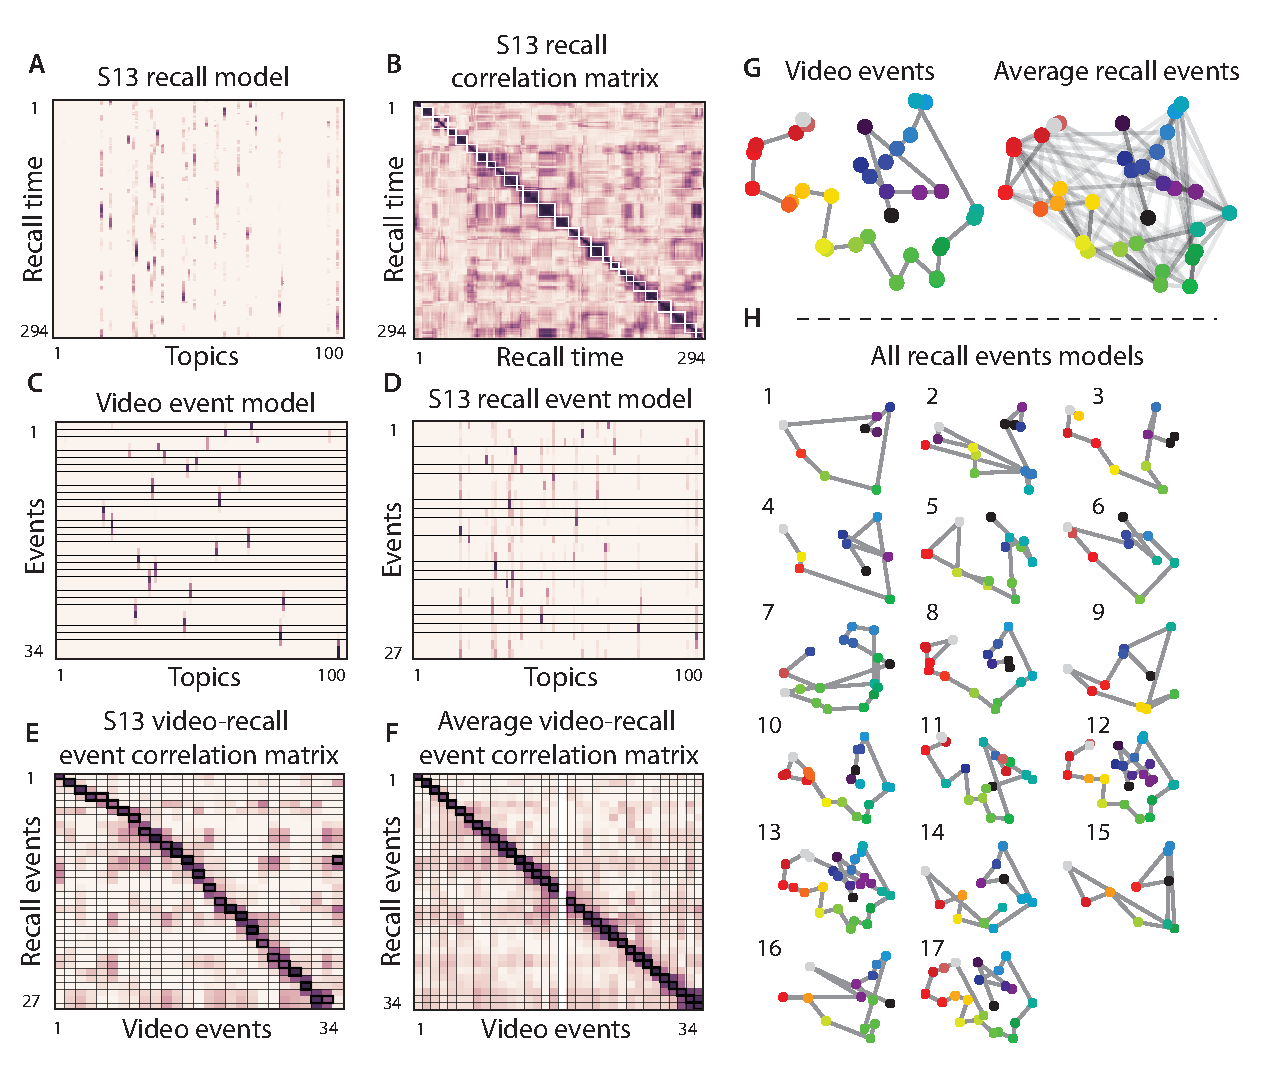
\includegraphics[width=.75\textwidth]{figs/2_eventseg.pdf}
\caption{\label{fig:eventseg} Event segmentation analysis of the video and recall models. A. A recall-time (294) by topics (100) matrix representing a recall model for a single participant (participant \#13).  B. A recall-time (294) by recall-time (294) correlation matrix for participant \#13. The white squares along the diagonal outline events, i.e. neighboring timepoints with a stable and similar topic vector. C. An events (34) by topics (100) matrix where each row represents the average topic vector for each event in the video model.  D. An events (27) by topics (100) matrix where each row represents the average topic vector for each event in the recall model. E. A recall events (27) by video events (34) correlation matrix representing the `match' between each video and recall event. The black squares identify the video event with the highest correlation to a given recall event. F. A group averaged recall events (34) by video events (34) correlation matrix.  The black squares identify the video event with the highest correlation to a given average recall event. G. 2D embeddings (reduced with UMAP algorithm) of each participants' recall event model (example shown in D). Each dot represents a recall event and the connecting lines indicate the order of recall. Colors indicate the most likely video event that the participant was describing as determined by the video-recall matching model.  H. 2D embedding of video and average recall event models.  }
\end{figure}


\subsubsection{Naturalistic extensions of classic memory analyses}
s
Traditionally, a major limitation of 'naturalistic' memory experiments has been quantifying memory dynamics in a principled way.
In the next section, we extend a set of classic memory analyses that were originally designed to measure memory in 'free recall' list-learning experiments to naturalistic settings. Just like recall


\begin{figure}[t!]
\centering
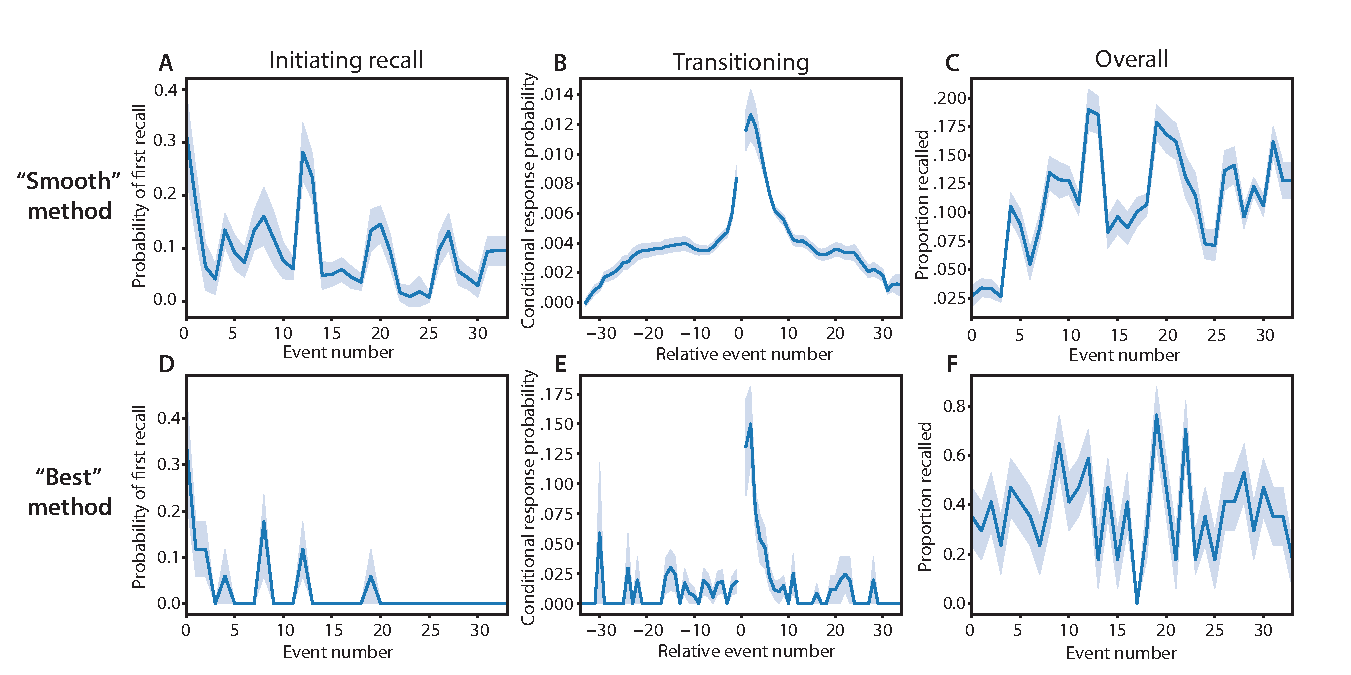
\includegraphics[width=1\textwidth]{figs/3_behav_eventseg.pdf}
\caption{\label{fig:behav}Naturalistic extensions of classic memory analyses. A-C use the `smooth' approach and D-F use the `best' approach (see Methods for details). A/D. The probability of first recall as a function of the serial position the the event during encoding. B/E. Given recall of event i, the probability that the next recalled item will be from serial position i \rpm~lag. C/F. Proportion recalled as a function of serial position. All error bars are the standard error of the mean derived from a bootstrap resampling procedure.
}
\end{figure}

\section{Methods}
\label{sec:methods}

% \subsection{Participants and Experimental Design}
% How much detail here? or just point to janice's paper?
%
% \subsubsection{Fitting a topic model from text descriptions of Sherlock}
% To quantify the flow of information from scene to scene, we used a topic model. A topic model estimates the most likely mixture of topics in a sample of text. First, the video was manually segmented into 1000 scenes, and a collection of descriptive features were manually transcribed.  For each scene, we considered the following features: scene details (i.e. a sentence or two describing what happened in that scene, space (indoor or outdoor), name of all the characters in the scene, name of the character in focus, name of the character speaking, location, camera angle, music presence, and words on the screen. We concatenated the text for all of these features within each segment, creating a 'bag of words' describing each scene. We then transformed the text descriptions into overlapping windows of 50 scene segments. For example, the first text sample comprised the text from the first 50 segments, the second comprised the text from n+1:n+51, and so on. We trained our model using these overlapping text samples using scikit-learn's `CountVectorizer' and `LatentDirichletAllocation' classes.  First, the text was transformed into a vector of word counts (default scikit-learn parameters). This gave a word count vector for each scene in the video.  Then, the word count vectors were used to fit a topic model (number of topics=100, method=batch).
%
% \subsubsection{Projecting the video and verbal recall into a common space}
% We used the model described above to transform the video text descriptions and verbal recall transcripts into a common space.  We created the video model by transforming exactly the same text (overlapping scene descriptions) with the topic model, resulting in a scene (1000) by topic (100) matrix that summarized the topics in each scene (Fig. \ref{fig:model}a). The scene descriptions often spanned multiple timepoints (i.e. TRs). To account for this, we expanded the video model by copying the rows of the model for as many timepoints that the scene description spanned. After this expansion, the shape of the model was the length of the duration of the video (1976 TRs).
%
% To create the recall models, for each participant we tokenized the recall transcript into a list of sentences and then mapped the list to overlapping windows of 10 sentences.  We transformed the list of overlapping recall sentences using the model that was trained on the video text. The result of this was a matrix (\# of sentences by 100 topics) that represented the most likely mixture of topics for a given chunk of sentences. We resampled the recall model to be the same length as the video model (1976 samples). The result was 17 participant-specific recall models (1976 timepoints by 100 topics). Intuitively, if the recall transcript for a given participant correctly described each video scene in order, the video and recall models should match closely.  However, if the scenes were recalled out of order, omitted, or described using language that was very different from the video scene descriptions, the video and recall models would look very different. Figure \ref{fig:model}b shows the group average recall model. Qualitatively, the two matrices appear to be similar. Our next set of analyses sought to quantify this relationship.
%
% To quantify the similarity between the movie and recall models, for each participant we correlated every moment of the video model with every moment of the recall models, resulting in a timepoints (1976) by timepoints (1976) correlation matrix for each participant.  The individual matrices for each participant can be seen in Supp Fig. X and the group average is displayed in \ref{fig:model}c.
%
% \subsubsection{Estimating the number of recall events for each participant}
% Our metric for choosing k was to select the value that maximized the ratio of the average `within-event' correlation (i.e. blocks of time the model identified as an event) and the average `across-event' correlation.
%
% \subsubsection{Characterizing memory performance}
% We used a few different metrics to assess memory that were all designed to capture the relationship between the video and recall models.  First, to get a general sense for the match between the video and recall matrices, we vectorized the the matrices and correlated them.  This resulted in a single number representing how well a given participant recalled the video. To get a temporally dynamic measure of memory, for each participant we computed the pairwise correlation between matching video/recall timepoints.  This allowed us to assess memory for individual moments of the video. Finally to get a more nuanced representation of memory for the video, we computed a video/recall model correlation matrix for each participant. These timepoint (1976) by timepoint (1976) matrices represent the correlation between every moment of the video model and every moment of the recall model. To provide some intuition, if a participant recalled every scene at the same rate and in exactly the same order as the video, we would expect high correlation values along the diagonal of this matrix. However, if a participant recalls the scenes out of order, or at different rates for different scenes, this will result in high values off the diagonal.

\subsection{References}

LaTeX automatically generates a bibliography in the APA style from your .bib file. The citep command generates a formatted citation in parentheses \citep{Lamport1986}. The cite command generates one without parentheses. LaTeX was first discovered by \cite{Lamport1986}.

% \subsection{Tables and Figures}

% Use the table and tabular commands for basic tables --- see Table~\ref{tab:widgets}, for example. You can upload a figure (JPEG, PNG or PDF) using the files menu. To include it in your document, use the includegraphics command as in the code for Figure~\ref{fig:frog} below.



\bibliography{memlab}

\end{document}

%
% Please see the package documentation for more information
% on the APA6 document class:
%
% http://www.ctan.org/pkg/apa6
%
